\chapter{Implementacja systemu}
\thispagestyle{chapterBeginStyle}

	W tym rozdziale opisane są technologie i biblioteki użyte do stworzenia aplikacji, jak i schemat 
użytej bazy danych.



\section{Opis technologii}


\subsection{React Native}
	Aplikacja została napisana w bibliotece React Native \cite{React-Native}. Jest to framework
umożliwiający tworzenie aplikacji mobilnych, komputerowych oraz internetowych. React Native jest oparty
na bibliotece React.js \cite{React-Js}, stworzonej przez Jordana Walke, a rozwijanej przez
Meta Platforms Inc. oraz społeczność, i jej rozwój także jest nadzorowany przez tę firmę. Framework
jest dostępny na licencji MIT.

	Głównymi pojęciami potrzebnymi do tworzenia aplikacji w React Native są komponenty oraz stany.
Komponenty reprezentują nie tylko podstawowe składniki interfejsu graficznego, takie jak pola tekstowe czy 
przyciski, ale także zestawy składników realizujące określoną funkcję, np. plansza do gry lub
lista gier. Komponenty opierają się o stan, czyli zestaw informacji przechowywany w komponencie i
komunikowany do użytkownika za pomocą interfejsu. Framework odświeża wygląd interfejsu przy zmianie
stanu, która najczęściej następuje w wyniku interakcji użytkownika z interfejsem. Wtedy to dochodzi
do aktualizacji komponentów korzystających z danego stanu.

	Programowanie w React Native odbywa się za pomocą języka skryptowego JavaScript. Znak towarowy
należy do Oracle \cite{JS-Oracle}, standard jest utrzymywany przez ECMA \cite{JS-ECMA}, 
a uruchamiany jest na różnych silnikach rozwijanych zgodnie ze standardem 
(np. V8 \cite{JS-V8} od firmy Google, czy SpiderMonkey \cite{JS-SpiderMonkey} od Mozilli).


\subsection{Dodatkowe biblioteki}
	Do stworzenia aplikacji zostały wykorzystane biblioteki tworzone przez społeczność. Są to
między innymi:
\begin{itemize}
	\item React Native Elements \cite{RN-Elements} - biblioteka zawierająca podstawowe komponenty 
zgodne z Material Design
	\item React Native Navigation \cite{RN-Navigation} - biblioteka obsługująca nawigację między 
aktywnościami
	\item React Native SQLite Storage \cite{RN-SQLite} - biblioteka pozwalająca korzystać z lokalnej
bazy SQLite
	\item React Native Zoomable View \cite{RN-Zooming} - biblioteka dodająca komponent obsługujący 
przybliżanie ekranu
\end{itemize}


\section{Baza danych}
	Dane aplikacji są przechowywane w bazie danych opartej na systemie SQLite. Schemat bazy jest
przedstawiony na diagramie poniżej.

\begin{figure}[!htb]
    \centering
    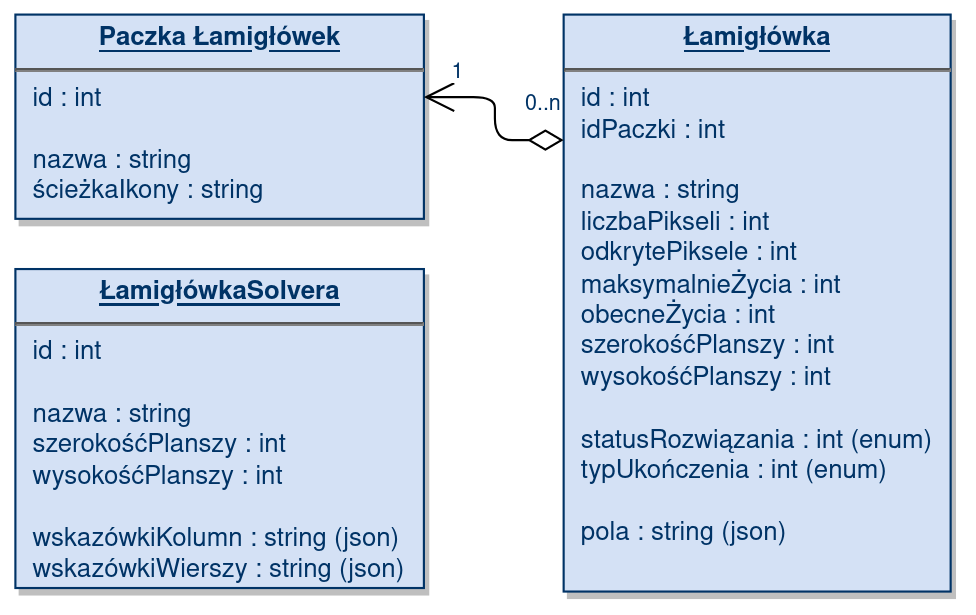
\includegraphics[width=\textwidth]{images/db_diagram.png}
    \caption{Diagram bazy danych}
\end{figure}

	Baza składa się z 3 tabel: paczek, łamigłówek i łamigłówek solvera. Paczki zawierają jedynie
niezbędne dane do reprezentacji grupy łamigłówek, czyli nazwa i ikona. W tabeli łamigłówek zawarte
są proste dane takie jak nazwa, maksymalna ilość żyć (ilość błędów, po których się przegrywa).
Przechowywane są tam również informacje o stanie gry, tj. \texttt{statusRozwiązania} — łamigłówka
nierozpoczęta i nierozwiązana, łamigłówka rozpoczęta, łamigłówka rozwiązana — oraz \texttt{typUkończenia} — łamigłówka nieukończona bez przegranej, łamigłówka nieukończona z przegraną, łamigłówka ukończona
bez przegranej, łamigłówka ukończona z przegraną. Pod zmienną \texttt{pola} przechowywana jest lista
pól wraz z ich stanami, pod postacią stringa w formacie JSON. Tabela łamigłówek solvera także zawiera
łamigłówki, ale w innej formie: łamigłówka zapisana jest jako listy wskazówek w formacie JSON oraz dane
do identyfikacji, np. nazwa czy wielkość planszy.
